\section{Linguistic tools}

One of the main parts of ReProTool project is an automatic text analyse. This part allows user to skip long-lasting manual annotation by pushing a button. This chapter describes implementation of linguistics analyse in ReProTool project and its linguistics background.

\subsection{Introduction}
Process of linguistics analyse gets natural language sentences as an input and returns analyzed usecases as is shown at figure \ref{fig:LinguisticsAnalyseSmall}. Whole process is divided into two parts: process of parsing and core analyse. Parsing contains main linguistics operations whitch are tokenization, tagging, parsing and lemmatization. Core work of parsing process is done by popular external linguistic analyse tools described in section \ref{sec:externaltools}. Core analyse converts parsed sentence trees with annotations into a usecases model ??. This process is described in more detail in section \ref{sec:analysis}. % TODO \ref{sec:usecasemodel}

Each implementation of any analyse brings problem of measuring success. We have put together a dataset of nearly tree hundred of sentences. These sentences contain the most commom use cases operations. All these sentences were manually anotated and analysed. In section \ref{sec:benchmark} is described our benchmark solution with actual results.

\begin{figure}[h]
  \centering
  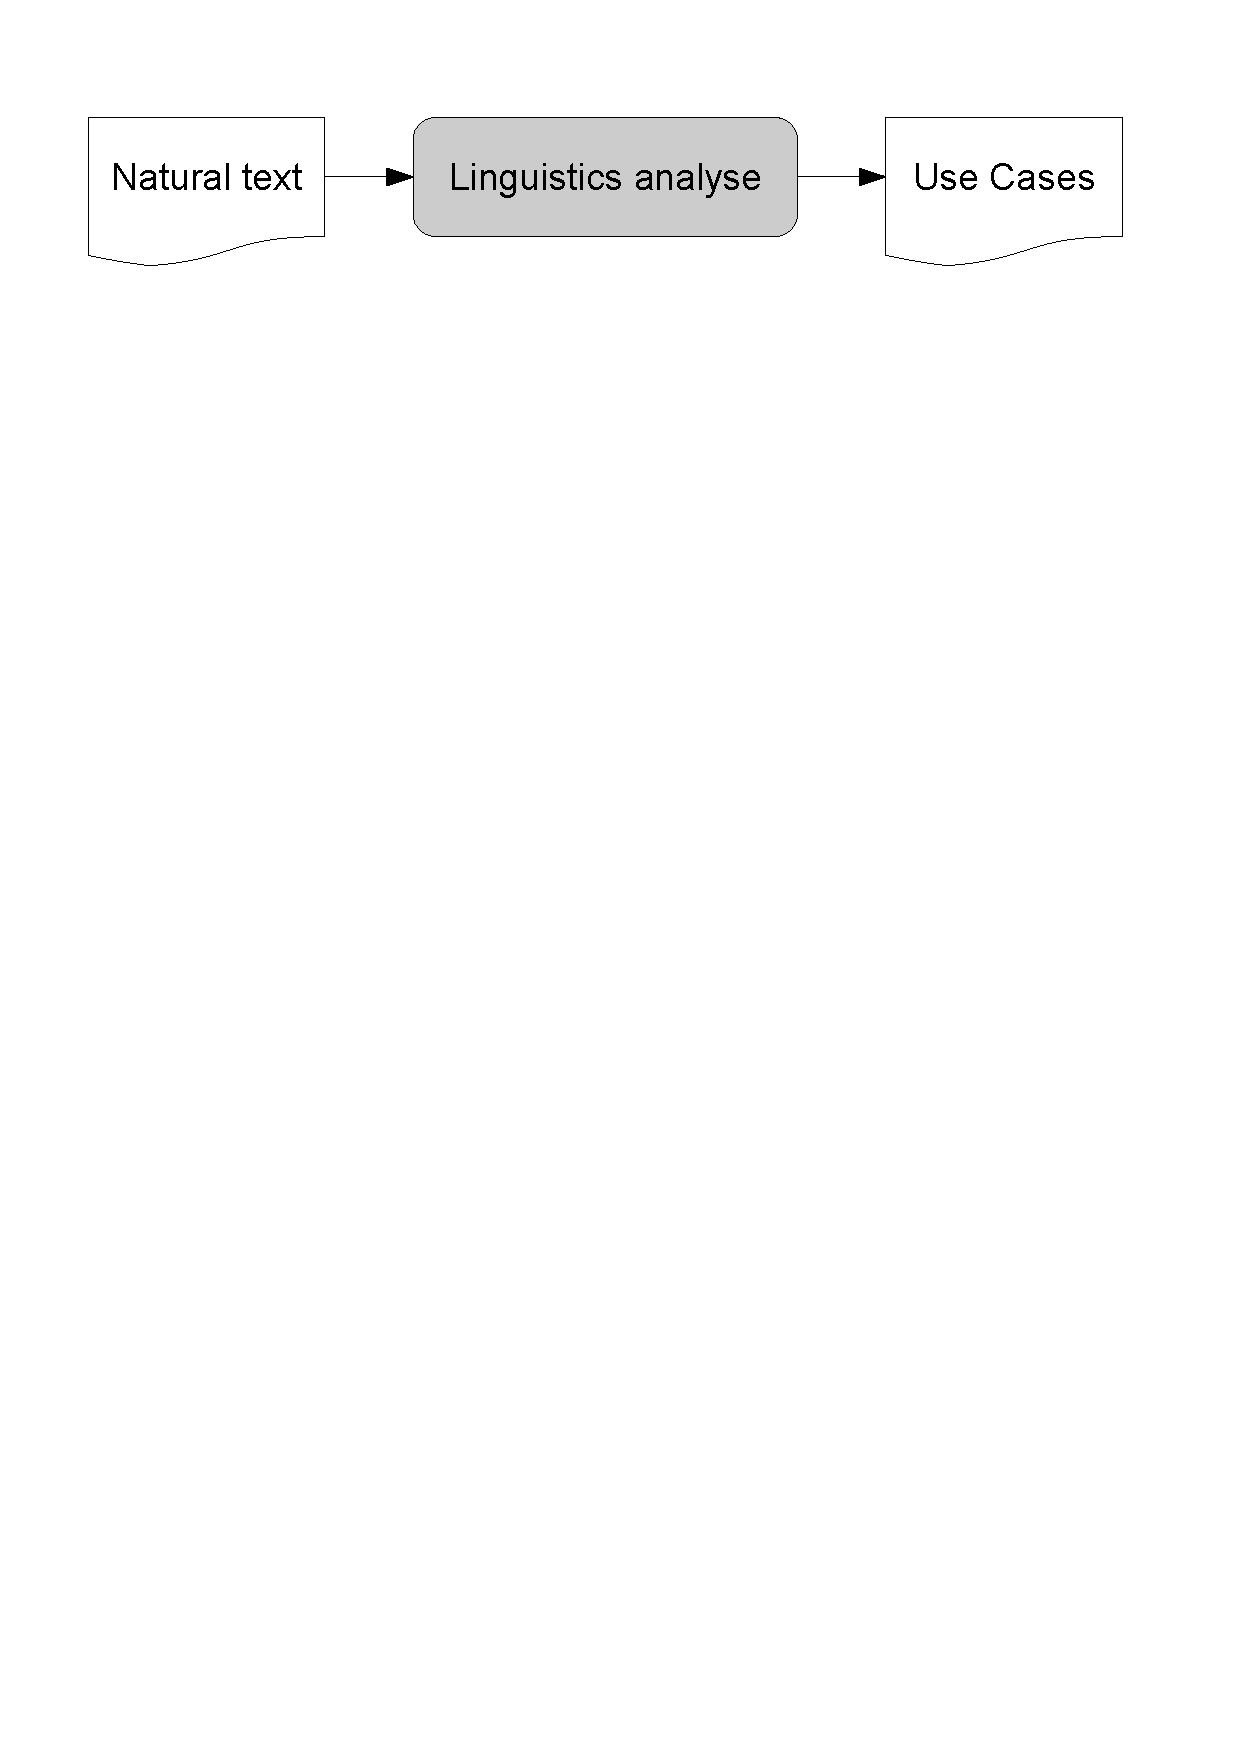
\includegraphics[height=30pt]{images/LinguisticsAnalyseSmall}
  \caption{Process of sentence analysis}
  \label{fig:LinguisticsAnalyseSmall}
\end{figure}

\subsection{Linguistics background}

Main goal of linguistic analyse in our porject is to identify important words in a sentence. These words are mainly constituents.

\begin{itemize}
\item {\bf Subject} main subject of the sentence
\item {\bf Main verb} verb wearing meaning
\item {\bf Representative object} main subject of sentence action
\item {\bf Indirect object} an actor usually owning representative object
\end{itemize}

\subsubsection{Deriving rules}

\subsection{External tools}
\label{sec:externaltools}

\begin{itemize}
\item MXPOST tagger \href{http://www.inf.ed.ac.uk/resources/nlp/local_doc/MXPOST.html}{Java implementation of MXPOST tagger}
\item Dan Bikel's Multilingual Statistical Parsing Engine \href{http://www.cis.upenn.edu/~dbikel/software.html#stat-parser}{Dan Bikel’s Home Page}
\item Mate-tools lemmatizer \href{http://code.google.com/p/mate-tools/}{Tools for Natural Language Analysis}
\end{itemize}

\subsection{Analysis}
\label{sec:analysis}

\begin{figure}[h]
  \centering
  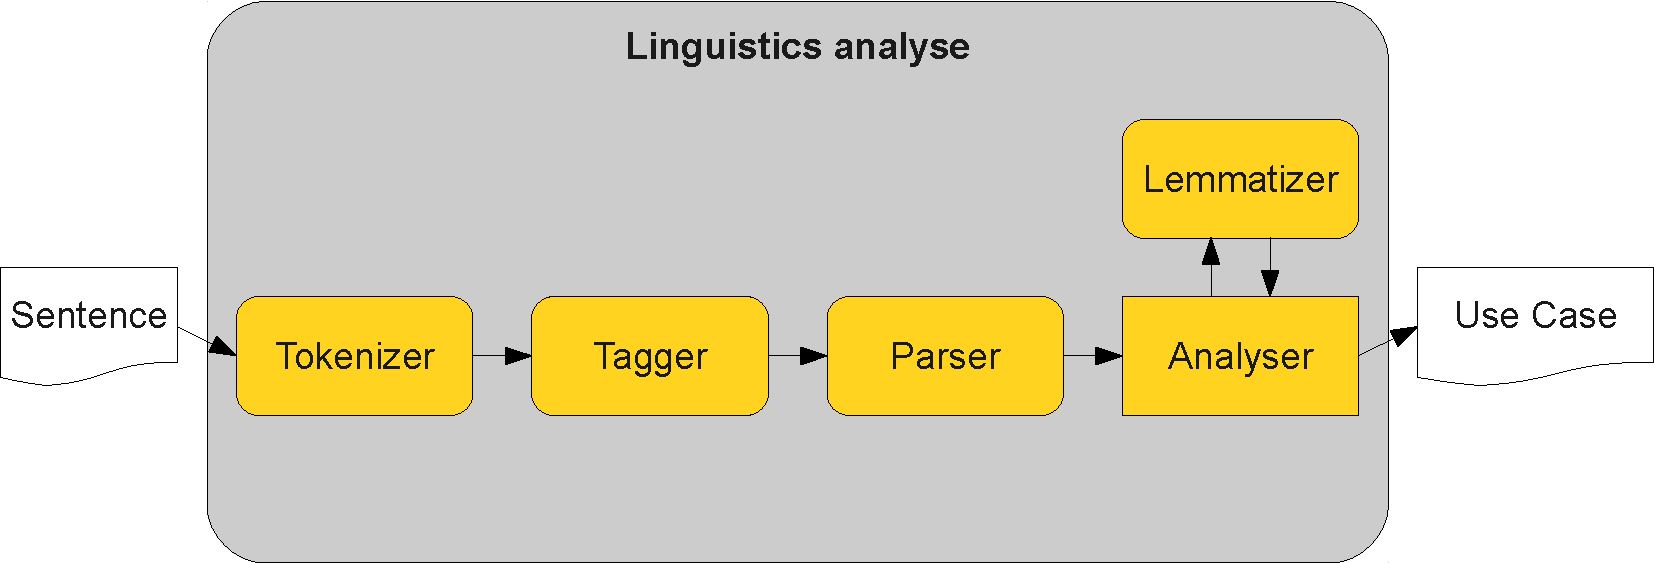
\includegraphics[height=300pt]{images/LinguisticsAnalyse}
  \caption{Process of sentence analysis}
  \label{fig:LinguisticsAnalyse}
\end{figure}

\subsubsection{Parsing}

\begin{figure}[h]
  \centering
  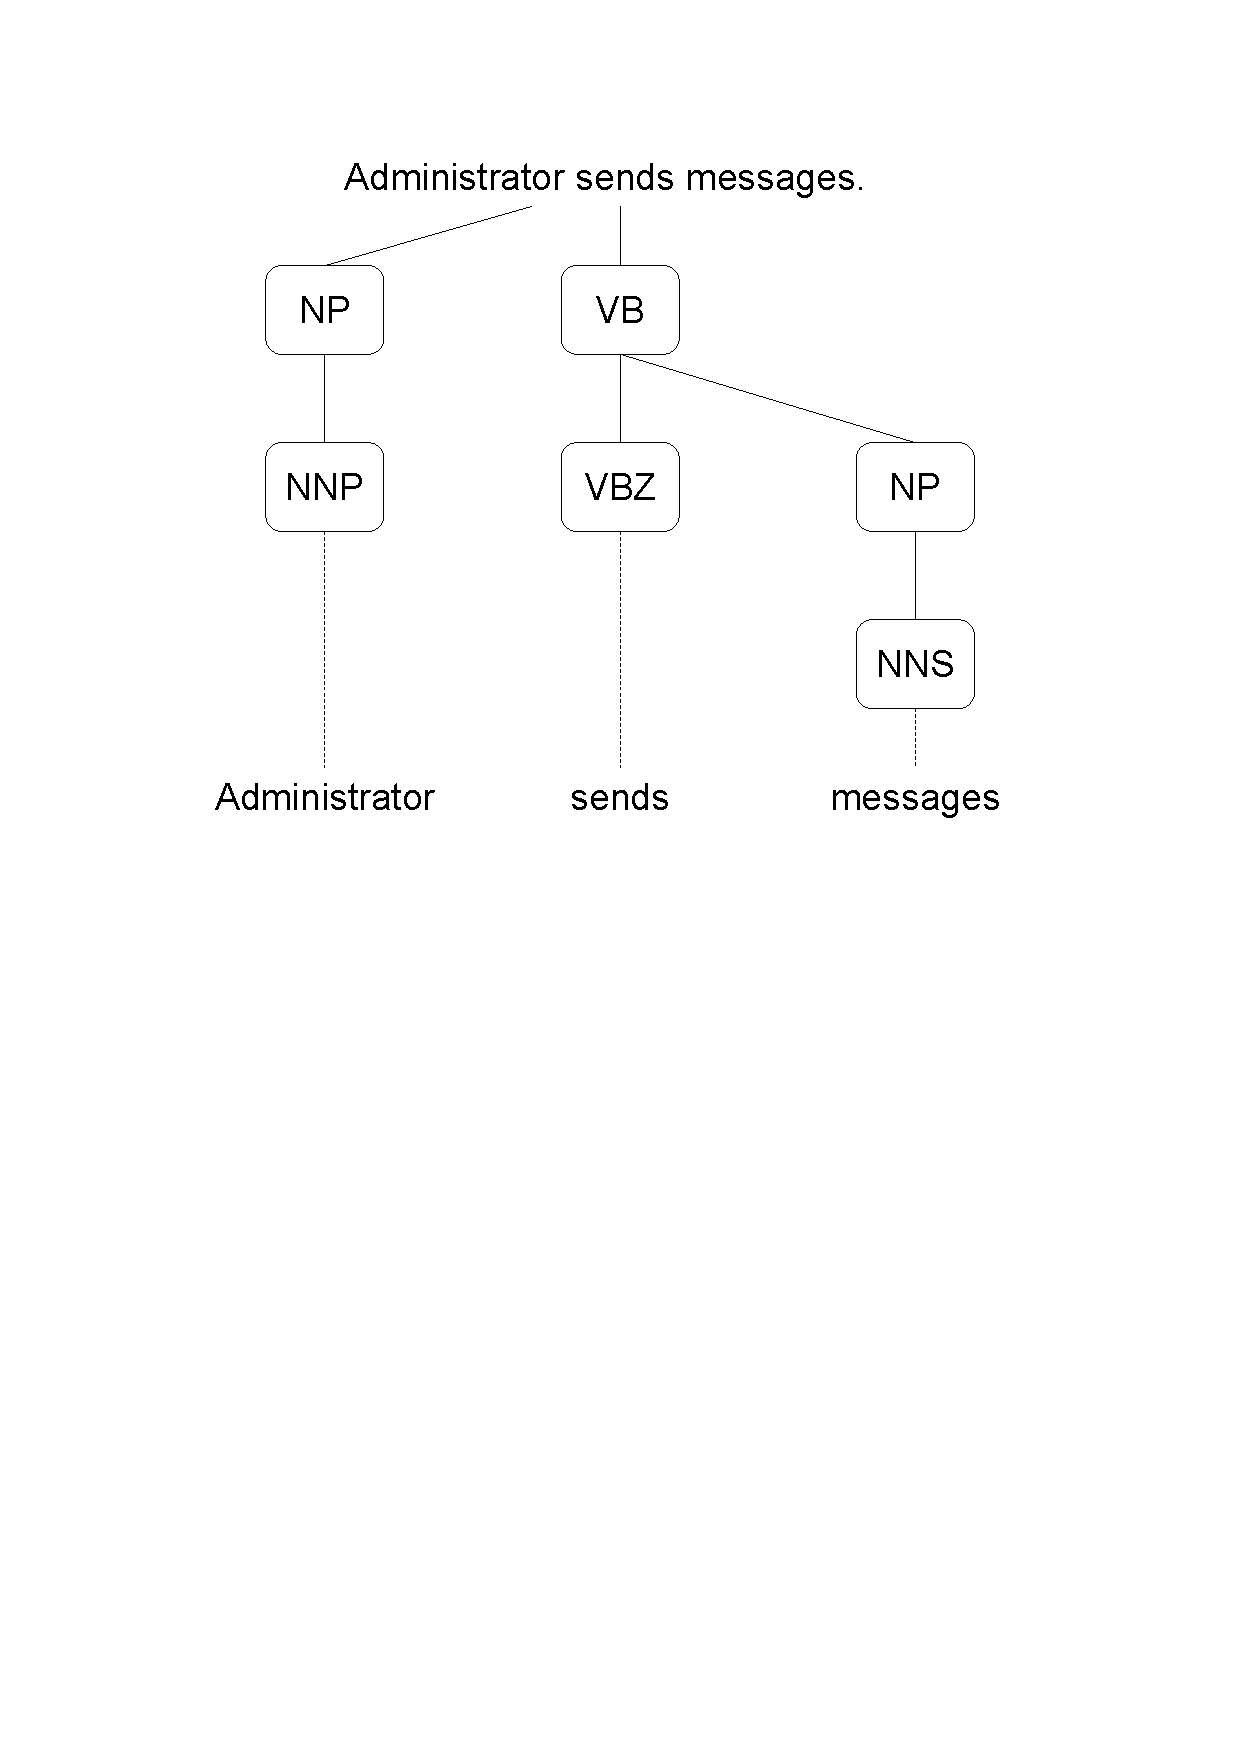
\includegraphics[height=300pt]{images/ParsedTree}
  \caption{Parsed tree of sentence "Administrator sends messages".}
  \label{fig:ParsedTree}
\end{figure}

\begin{figure}[h]
  \centering
  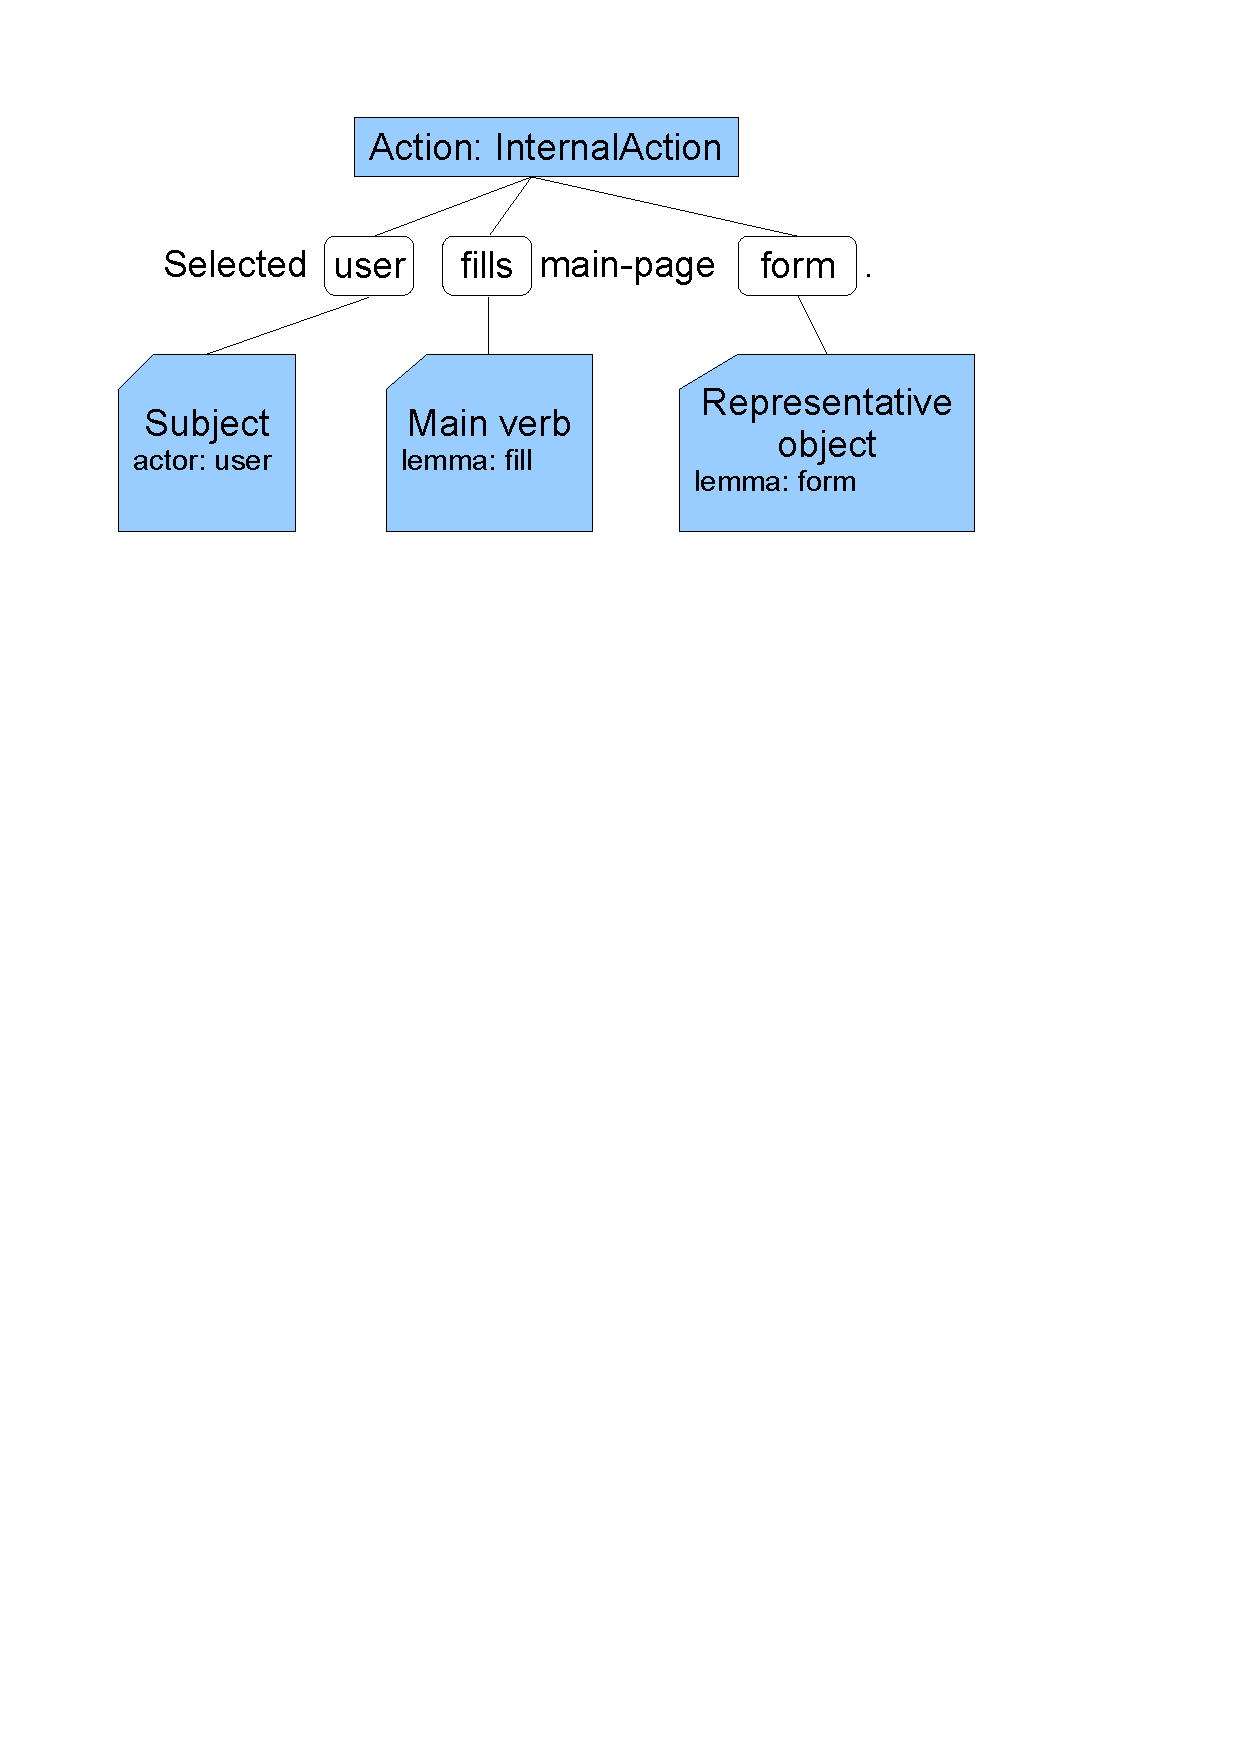
\includegraphics[width=400pt]{images/InternalActionExample}
  \caption{Example of internal action analyse result.}
  \label{fig:InternalActionExample}
\end{figure}


\subsection{Benchmark}
\label{sec:benchmark}

Main usecase benchmark dataset:

\href{http://www2.put.poznan.pl/en}{Poznan University of Technology}

\href{http://www.se.cs.put.poznan.pl/knowledge-base/software-projects-database/use-cases-database-ucdb/use-cases-database-ucdb}{Use Cases Database (UCDB)}

\href{http://ucdb.cs.put.poznan.pl/benchmark/2.f.n/srs/index.html}{Admission System version 2.0F (quantitative)}


\subsubsection{Implementation}

\begin{table}[ht]   % or b
\begin{center}
    \begin{verbatim}
SUBJECTS: Count: 21 Found: 19 | 90,5%
RPT6: input subjectNumber: 6 output subjectNumber: 1
MOD1_UC1_7: input subjectNumber: 0 output subjectNumber: 3
VERBS: Count: 21 Found: 20 | 95,2%
MOD1_UC1_5: input verbLemma: "verify" output verbLemma: "be"
INDIRECT_OBJECTS: Count: 21 Found: 20 | 95,2%
LING2: input indirectObjectNumber: 8 output indirectObjectNumber: 0
OBJECTS: Count: 21 Found: 11 | 52,4%
RPT8: input objectNumber: 2 output objectNumber: 0
LING1: input objectNumber: 8 output objectNumber: 4
MOD1_UC1_7: input objectNumber: 3 output objectNumber: 0
MOD1_UC1_8: input objectNumber: 0 output objectNumber: 5
TOTAL: Count: 84 Found: 70 | 83,3%
    \end{verbatim}
  \caption{Example output from benchmark plugin}
  \label{tab.benchmarkexample}
\end{center}
\end{table}   
      
\subsubsection{Results}
                        
\begin{table}[ht]   % or b
\begin{center}
    \begin{tabular}{|l|c|}
      \hline
      {\bf Section} & {\bf Accuracy} \\
      \hline
      Subjects               & 91.5\% \\
      Verbs                  & 80.1\% \\
      Representative objects & 70.3\% \\
      Indirects objects      & 70.5\% \\
      Actions                & 20.8\% \\
      \hline
      {\bf Total} & {\bf 80.2\%} \\
      \hline
    \end{tabular}
 \caption{Overall results of analyse benchmark on dataset data.csv (269 sentences)}
 \label{tab.benchmark}
\end{center}
\end{table}

